% THIS IS AN EXAMPLE DOCUMENT FOR VLDB 2012
% based on ACM SIGPROC-SP.TEX VERSION 2.7
% Modified by  Gerald Weber <gerald@cs.auckland.ac.nz>
% Removed the requirement to include *bbl file in here. (AhmetSacan, Sep2012)
% Fixed the equation on page 3 to prevent line overflow. (AhmetSacan, Sep2012)

\documentclass{vldb}
\usepackage{graphicx}
\usepackage{caption}
\usepackage{subcaption}
\usepackage{caption}
\usepackage{subcaption}
\usepackage{hyperref,array,color,balance,multirow}
\usepackage{balance,float,url,amsfonts,alltt}
\usepackage{mathtools,rotating,amsmath,amssymb}
\usepackage{color,cite,ifpdf,fancyvrb,array,listings}
\usepackage{algorithm,algpseudocode}
\usepackage{tabularx}
\usepackage{natbib}
\usepackage{hyperref,array,color,balance,multirow}
\usepackage{balance,float,url,amsfonts,alltt}
\usepackage{mathtools,rotating,amsmath,amssymb}
\usepackage{color,cite,ifpdf,fancyvrb,array,listings}
\usepackage{algorithm,algpseudocode}
\usepackage{tabularx}
\usepackage{natbib}
\usepackage{balance}  % for  \balance command ON LAST PAGE  (only there!)


\begin{document}

% ****************** TITLE ****************************************

\title{Optimizing Coordinate Descent over Normalized Data in Column Stores}

% possible, but not really needed or used for PVLDB:
%\subtitle{[Extended Abstract]
%\titlenote{A full version of this paper is available as\textit{Author's Guide to Preparing ACM SIG Proceedings Using \LaTeX$2_\epsilon$\ and BibTeX} at \texttt{www.acm.org/eaddress.htm}}}

% ****************** AUTHORS **************************************

% You need the command \numberofauthors to handle the 'placement
% and alignment' of the authors beneath the title.
%
% For aesthetic reasons, we recommend 'three authors at a time'
% i.e. three 'name/affiliation blocks' be placed beneath the title.
%
% NOTE: You are NOT restricted in how many 'rows' of
% "name/affiliations" may appear. We just ask that you restrict
% the number of 'columns' to three.
%
% Because of the available 'opening page real-estate'
% we ask you to refrain from putting more than six authors
% (two rows with three columns) beneath the article title.
% More than six makes the first-page appear very cluttered indeed.
%
% Use the \alignauthor commands to handle the names
% and affiliations for an 'aesthetic maximum' of six authors.
% Add names, affiliations, addresses for
% the seventh etc. author(s) as the argument for the
% \additionalauthors command.
% These 'additional authors' will be output/set for you
% without further effort on your part as the last section in
% the body of your article BEFORE References or any Appendices.

\numberofauthors{4} %  in this sample file, there are a *total*
% of EIGHT authors. SIX appear on the 'first-page' (for formatting
% reasons) and the remaining two appear in the \additionalauthors section.

\author{
% You can go ahead and credit any number of authors here,
% e.g. one 'row of three' or two rows (consisting of one row of three
% and a second row of one, two or three).
%
% The command \alignauthor (no curly braces needed) should
% precede each author name, affiliation/snail-mail address and
% e-mail address. Additionally, tag each line of
% affiliation/address with \affaddr, and tag the
% e-mail address with \email.
%
}
% There's nothing stopping you putting the seventh, eighth, etc.
% author on the opening page (as the 'third row') but we ask,
% for aesthetic reasons that you place these 'additional authors'
% in the \additional authors block, viz.

% Just remember to make sure that the TOTAL number of authors
% is the number that will appear on the first page PLUS the
% number that will appear in the \additionalauthors section.


\maketitle

\begin{abstract}

\end{abstract}

\newpage % space reserved for abstract


\section{Introduction}

\newpage % space reserved for introduction

\section{BACKGROUND AND PRELIMINARIES}
We provide a brief introduction to GLMs, CD and MonetDB. For a deeper understanding and interests, we refer the 
readers to \cite{hastie}\cite{Mitchell}\cite{Wright1}\cite{Boncz}, we use the same notation used in \cite{Kumar}.

\begin{table}
\begin{tabular}{c}
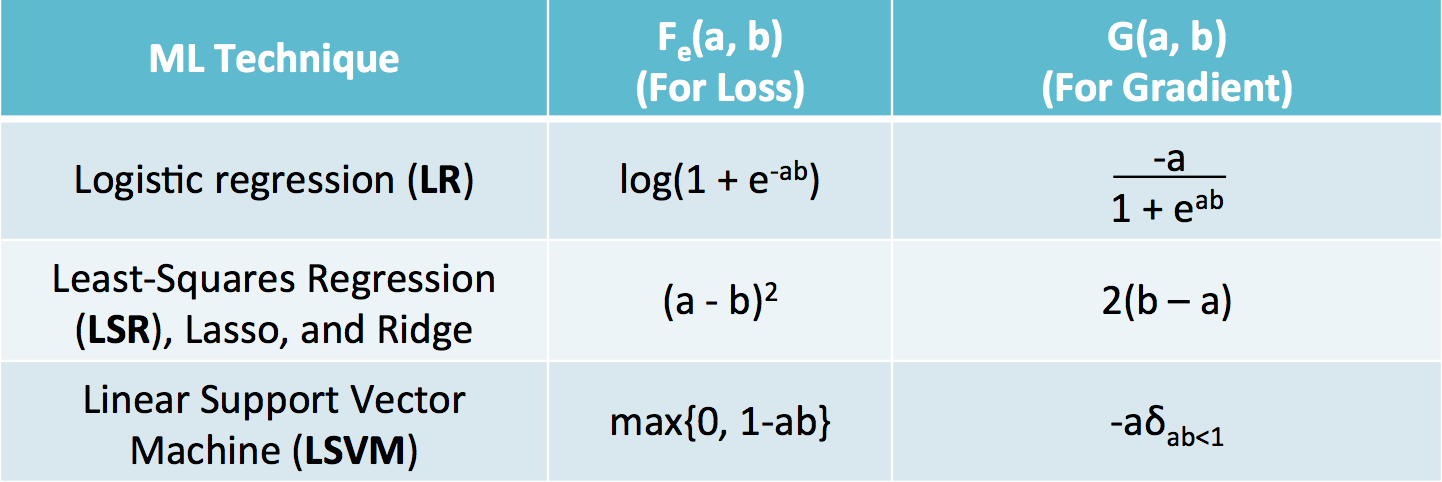
\includegraphics[width=3.3in]{figs/glms.png}
\end{tabular}
\vspace{-4mm}
\caption{GLMs and their functions.}
\label{tab:glms}
\end{table}

\subsection{Generalized Linear Models (GLMs)}
Consider a matrix $\textbf{X}$ with dimension $n \times d$ representing a dataset including n samples
and each sample has d features. Then the $i_{th}$ row of matrix $\textbf{X}$(namely $\textbf{X}_{(i,)}$) represents the $i_{th}$
sample in the dataset with its corresponding d features; the $j_{th}$ column of matrix $\textbf{X}$(namely $\textbf{X}_{(,j)}$)
represents the $j_{th}$ feature of all examples in the dataset. $Y$ is a n-dimensional vector representing numerical
targets for all samples in the datasets. For instance, $Y_{i}$ is a numerical target for $\textbf{X}_{(i,)}$. $Y_{i} \in \mathbb{R}$ considering 
regression (continuous target values). For discrete target values, however, $Y_{i}$ represents the numerical value
representing the defined class, such as classification in binary class, $Y_{i}\in{\{-1,1\}}$.  GLMs make 
the assumption that the data in dataset could be distributed in different classes (discrete target values for classification) 
or assigned approximated values (continuous target values for regression) by a hyperplane. Such hyperplane is called 
``model", and the ultimate goal is to use the given dataset $\textbf{X}$ to compute the model $\textbf{W} \in \mathbb{R}^d$.
To evaluate how accurate the model is, a \textit{linearly-separable} objective function is given to compute the
\textit{loss} of the model $\textbf{W} \in \mathbb{R}^d$ on the data:
$F(\textbf{W}) = \sum_{i=1}^{n}{F_e(Y_i,  \textbf{W}^T\textbf{X}_{(i,)}^T)}$.
Applying proper ML algorithm to find the optimal solution for model $\textbf{W}\in \mathbb{R}^d$ to minimize the loss function
is the ultimate goal. The corresponding mathematical statement is:
find a vector $\textbf{W}^*\in \mathbb{R}^d$ s.t.,  $\textbf{W}^* = argmin_{\textbf{W}^*}F({\textbf{W}})$.

\subsection{Coordinate Descent(CD)}
\textit{Coordinate Descent}(CD)  is a column-friendly algorithm (fetch one column each time for a single coordinate update), thus we consider CD in 
column stores taking advantage of the fact that the data is stored in columns in the column-oriented DBMS (specifically we use MonetDB as paradigm in our work). 
%Continue Explanation for Coordinate Descent 
%Paper of Stephen Wright should be referred

Here, we first just present the most basic version of CD for simplicity. The algorithm just updates one coordinate each time 
regarding other coordinates as fixed in each iteration. However, as noted in \cite{Wright}, most applications in real life use \textit{block coordinate descent} (BCD),
in which several coordinates regarded as one block are updated synchronously each time in each iteration regarding other ``blocks" are fixed 
instead of updating just a single coordinate each time. We will briefly discuss BCD in the extensional work part and it shows that our 
new-designed techniques will also have better performance improvement (in terms of speed-up) in BCD compared to the \textit{single coordinate descent} method.

CD is a simple algorithm to solve GLMs using iterative numerical optimization. CD initializes the model $\textbf{W}$ to some $\textbf{W}^{(0)}$, 
considering a single coordinate every time in each iteration, the algorithm assumes all other coordinates are fixed except for $\textbf{W}_j$, the $j_{th}$ entry in the model to be updated. Compute the partial gradient $\nabla F_j(\textbf{W})$ on the given dataset on coordinate $W_j$ (corresponding to $j_{th}$ feature) , where 
$\nabla F_j(\textbf{W}) = \sum_{i=1}^{n}{G(Y_i, \textbf{W}^T\textbf{X}_{(i,)}^T)}\textbf{X}_{(i,j)}$. And then updates the $j_{th}$ entry in the model as $W_j \leftarrow W_j - 
\alpha \nabla F_j(\textbf{W})$, where $\alpha > 0$ is the \textit{learning rate} (stepsize) parameter. Once after finishing the update of current coordinate, the algorithm goes into the updating process for the next coordinate in the model $\textbf{W}$. The coordinate descent that updates one single coordinate each time is also called 
\textit{stochastic coordinate descent} (SCD). SCD is outlined in Algorithm~\ref{alg:cd}. 

SCD updates the model repeatedly, i.e., over many \textit{iterations} (or \textit{epoches}), each of which requires at least one pass of data. The loss value typically decreases over iterations. The algorithm stops typically with some pre-defined conditions (i.e., specific number of iterations, the decrease of loss value across iterations). The learning rate parameter ($\alpha$) is typically selected using a line search method that potentially computes the loss many times. Conventionally, \textit{re-ordering} (shuffling) of data in the dataset is done in every iteration to reduce the \textit{influence} that might be caused by data ordering on learning process. However, many practical 
experiments show that one shuffling is good enough to mitigate the influence of data ordering, thus it is not necessary to shuffle the data in every iteration. We apply this 
idea in our implementations.

Here, we present the general version of CD algorithm which can be applied for all GLMs listed on Table~\ref{tab:glms}. H is $n \times 1$ \textit{residual vector}, which stores the $\textbf{W}^T\textbf{X}_{(i,)}^T$ for every $X_{(i,)}$ with current \textbf{W}. In some cases, it is possible to find the optimal $\textbf{W}_j$ mathematical expression. For reader's interests, we refer \cite{CMU}, which presents CD applied in LSR.

%Coordinate Descent Algorithm 
\begin{algorithm}[t]
\caption{Coordinate Descent (CD)}
\label{alg:cd}
\textbf{Inputs}: $\{{\textbf{X}, Y}\}$ (Data)
\begin{algorithmic}[1]
\State $k \leftarrow 0$, $r_{prev} \leftarrow$ null, $r_{curr} \leftarrow$ null,  $H \leftarrow \textbf{0}$, $\textbf{W} \leftarrow \textbf{0} $
\While {(Stop ($k$, $r_{prev}$, $r_{curr}$) = False)}
       \State $r_{prev} \leftarrow r_{curr}$
        \For{j = 1 to d}\Comment{1 pass over data}
                 \State $\nabla F_{j}^{k}(\textbf{W})\leftarrow \sum_{i=1}^n{G(Y_{i}, H_i )}X_{(i,j)}$   
		\State $\textbf{W}_j^{(k)} = \textbf{W}_j^{(k-1)} - \alpha \nabla F_{j}^{k}(\textbf{W})$   
		\State $H \leftarrow H+(\textbf{W}^{k}_{j}-\textbf{W}^{(k-1)}_{j})\times \textbf{X}_{(,j)} $
	\EndFor
	\State $r_{curr} \leftarrow  F_{k}$
	\State $k \leftarrow k+1$
\EndWhile
\end{algorithmic}
\end{algorithm}

\subsection{MonetDB}
We use MonetDB, an open-source column store, as the paradigmatic column-oriented DBMS in this paper. In order to give 
readers a better understanding of our work, we provide a brief introduction to MonetDB. Readers can also refer to \cite{Boncz}.

\begin{figure}[t]
    \centering
    \begin{subfigure}[b]{0.5\textwidth}
        \centering
        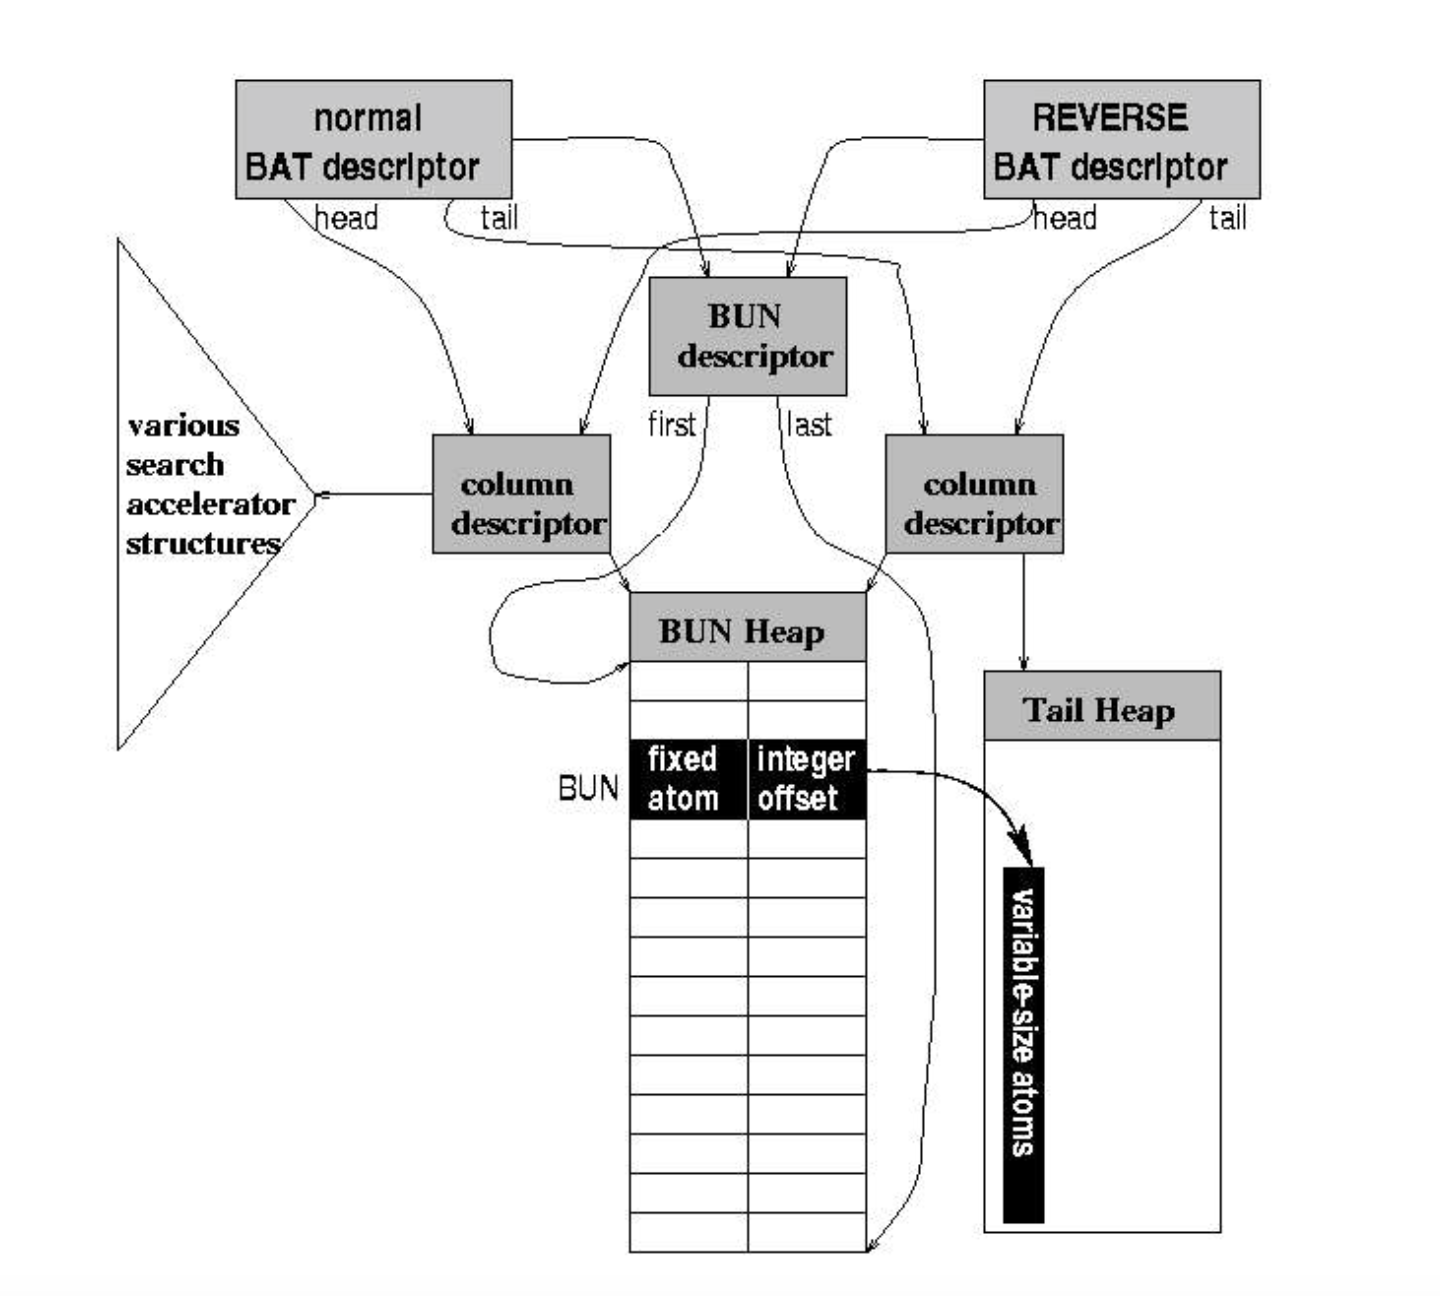
\includegraphics[height = 5cm]{figs/DS1.png}
        \caption{BAT Data Structure}
        \label{BAT}
    \end{subfigure}
    \begin{subfigure}[b]{0.4\textwidth}
        \centering
        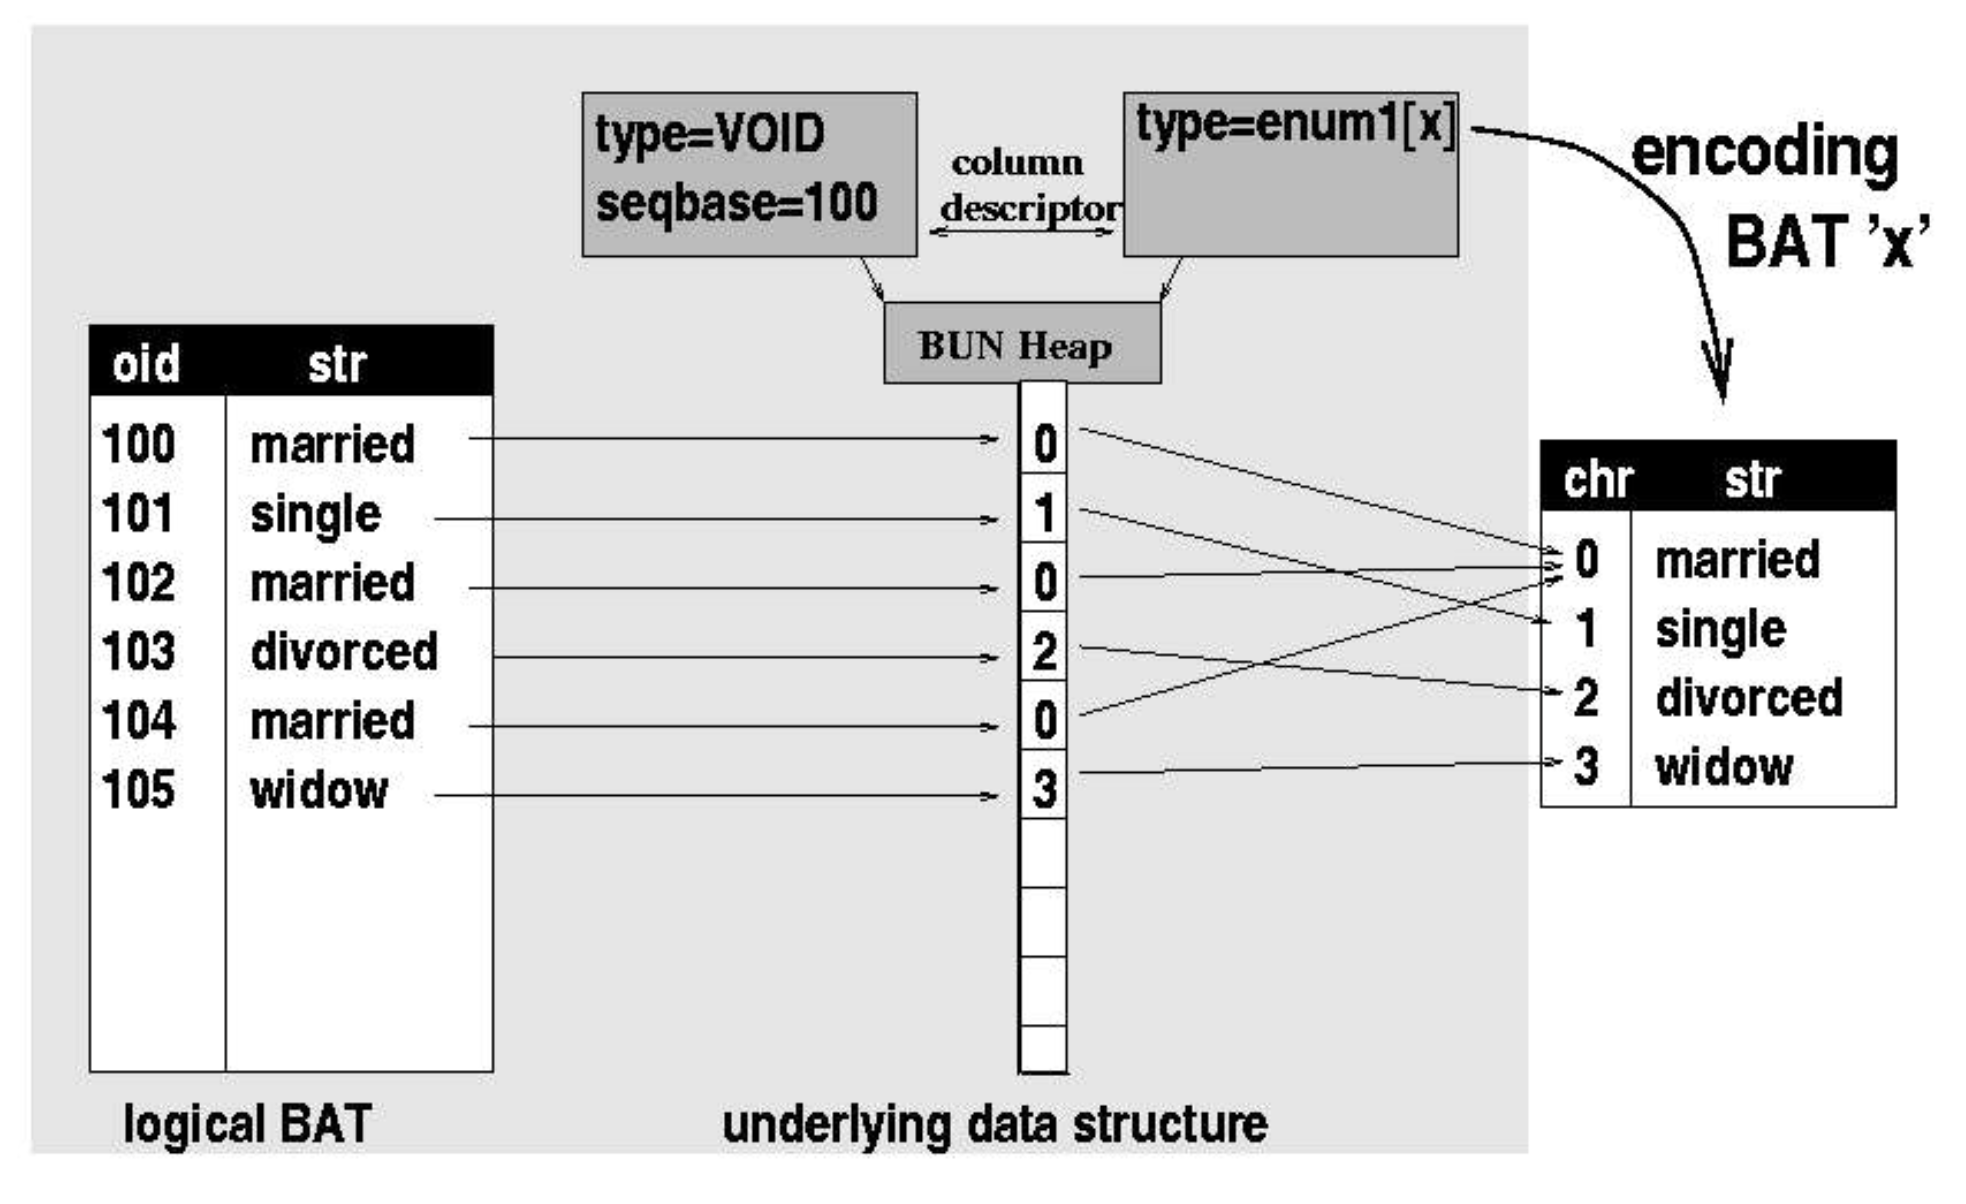
\includegraphics[height = 4cm]{figs/DS2.png}
        \caption{The logical mapping of BAT}
        \label{logical mapping}
    \end{subfigure}
    \caption{MonetDB Data Structure}
    \label{fig:ds}
\end{figure}

\subsubsection{Data Structure}
The data structure used in MonetDB is called \textit{binary association table} (BAT). Every column in the table is stored in a BAT. The single unit in BAT
is called \textit{binary unit} (BUN). The two columns of BAT is called \textit{BUN Heap} and the first column in BUN Heap is called \textit{head}, which 
stores \textit{objective identifier} (OID, used to refer the logical location of each tuple in the table); the second column in BUN heap is called \textit{tail}, which stores
the corresponding attribute (or feature). All BATs for the same table that store all different features have the same OID in the head columns in BUN Heaps.
Figure~\ref{fig:ds} shows the graphic depiction of BAT. 

\begin{figure}[H]
\centering
{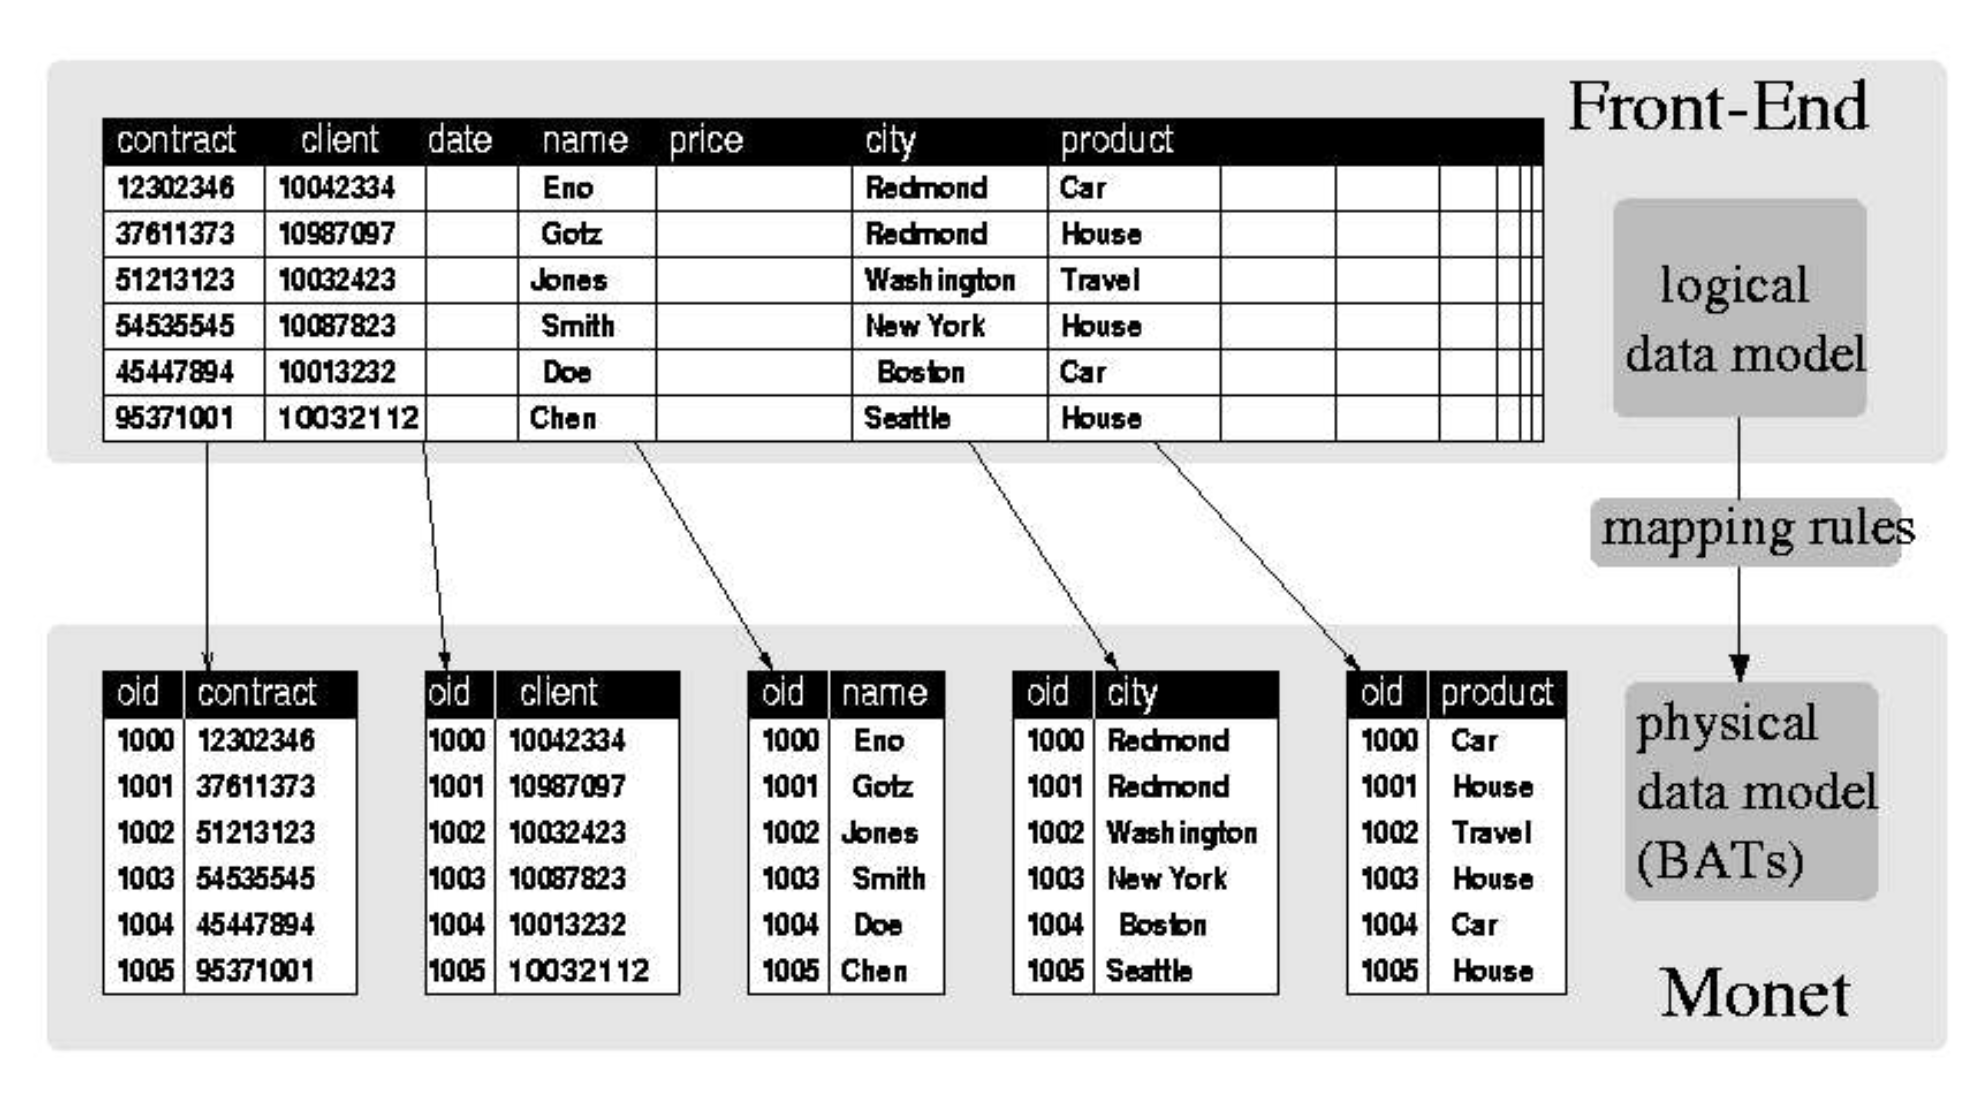
\includegraphics[natwidth=240bp,natheight=60bp, width=240bp]{figs/Mapping.png}}
\caption{Examples of storage of relations in MonetDB}
\label{fig:relation}
\end{figure}

\subsubsection{Storing Relations in MonetDB}
In Figure~\ref{fig:relation}, it shows how every attribute in the ``contract" table is stored in the BAT data structure in MonetDB. We can observe that different attributes 
on the same row in the ``contract" table have the same oid in different BATs, and this observation conforms to the description of BAT data structure given before. 
It should not be hard to conjecture that MonetDB uses oid to locate and fetch the data needed: once the oid for certain tuple in database
is known, all attributes in this tuple could be fetched in corresponding BATs using the oid as reference. What should be noticed here is that for different tables, 
the oid generated by the database system will be different (length, sequence). In other words, oid is unique for different tables and \textbf{No} same oid
can be or should be found in BATs for two different tables. Otherwise there will be conflicts and problems when fetching data in different tables but share the same oid.
%Exceptions could exist for oid uniqueness

\begin{figure}[H]
\centering
\begin{subfigure}{0.5\textwidth}
  \centering
  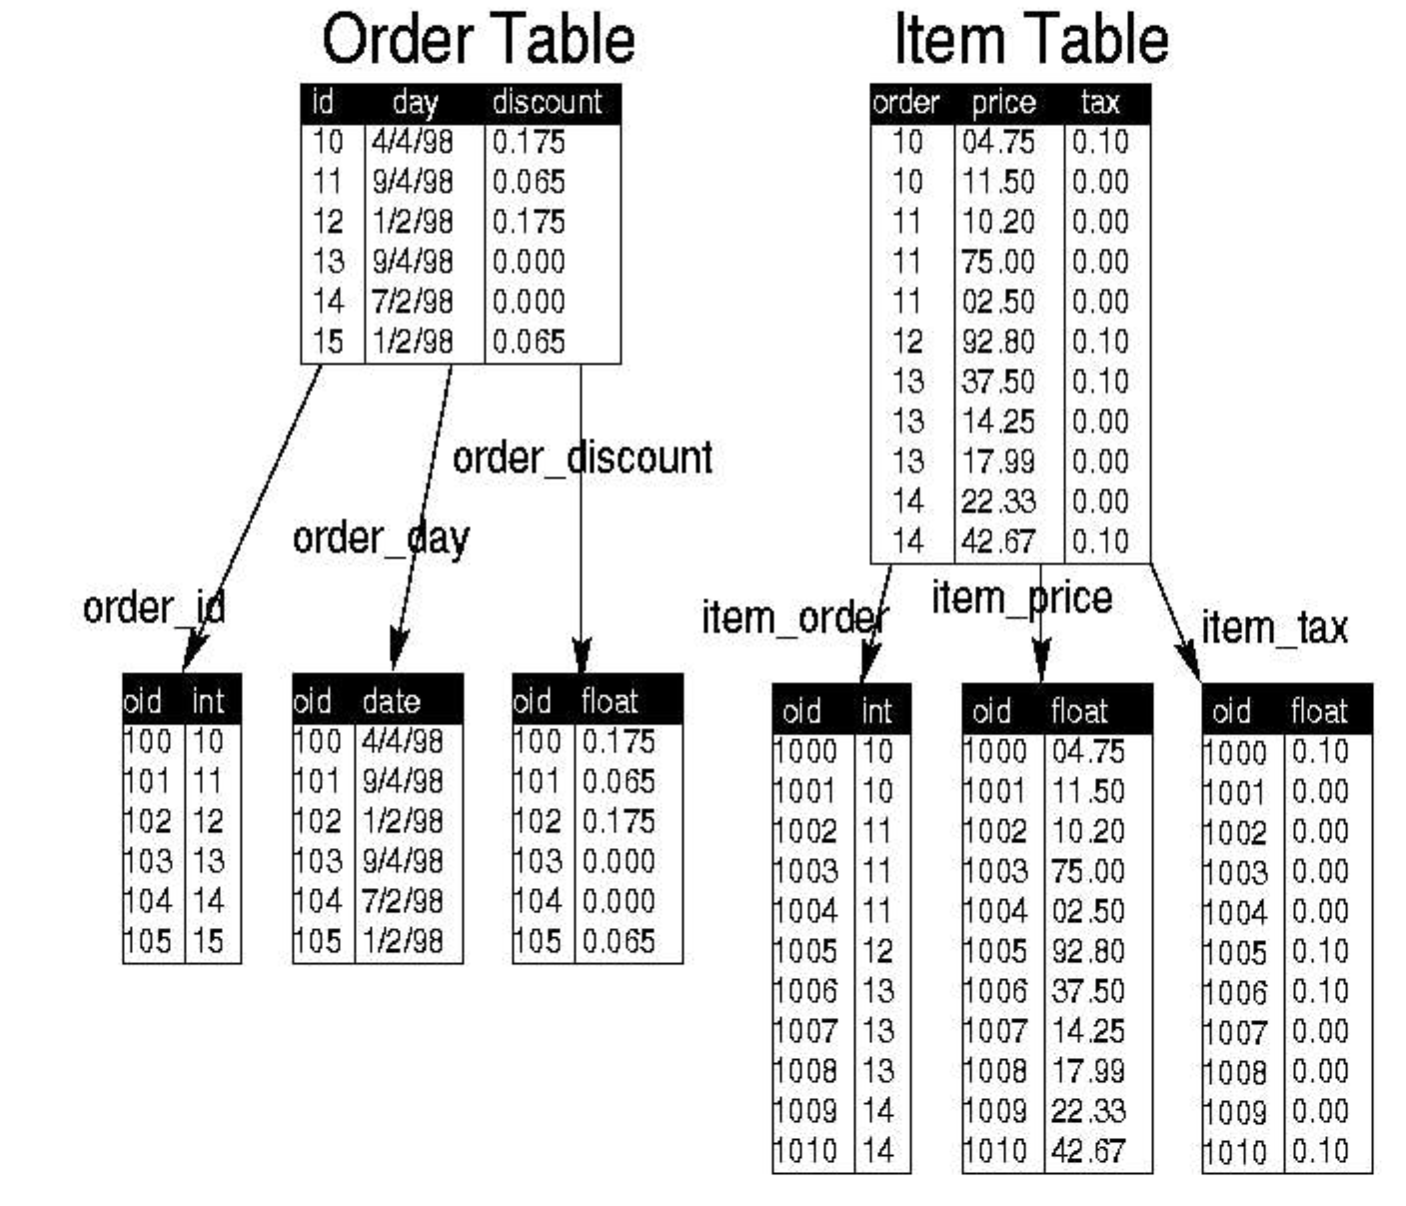
\includegraphics[width = 5cm, height = 5cm]{figs/SRMapping.png}
  \caption{BAT mapping of ``Order" and ``Item"}
\end{subfigure}
\begin{subfigure}{0.4\textwidth}
  \centering
  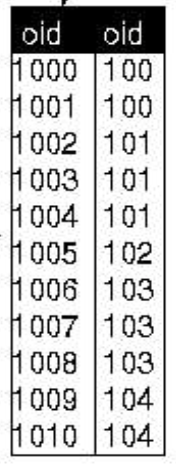
\includegraphics[width = 2cm, height = 5cm]{figs/OID_OID.png}
  \caption{oid-oid mapping}
\end{subfigure}
\caption{Relational mapping of ``Order" table and ``Item" Table}
\label{fig:relation example}
\end{figure}

\subsubsection{Examples of relational mapping}
Figure~\ref{fig:relation example} gives a general sense of relational mapping between two tables: let's say we want to join the ``Order" table and ``Item" table on order ``id".
then ``id" would be the primary key of ``Order" table and ``order" in ``Item" table is the foreign key refers to the order ``id" in ``Order" table. Looking at the order\_id and 
item\_order BATs in Figure~\ref{fig:relation example}(a), since the oids for all attributes are the same in the same tuple of the same table, once the oid-oid mapping of ``Order" and ``Item" is got, the join of ``Order" table and ``item" table can be completed by copying all the attributes to the corresponding position referred by oid following oid-oid mapping. The oid-oid mapping is shown in Figure~\ref{fig:relation example}(b). To get the oid-oid mapping, simple hash join is applied since only two BATs (primary key and foreign key) are needed (thus it is reasonable to assume that they can fit well in memory). We call this oid-oid mapping as ``key-foreign key mapping reference"(KKMR) and will use this notation in later sections.

% For consistency, we still use the same notations in problem statement in \cite{Kumar}.
% \paragraph*{Joins Before Learning}
\paragraph*{Problem Definition}
Suppose there are $n_S$ examples (tuples) in \textbf{S}, and $n_R$ tuples in \textbf{R}.
Assume that the feature vectors are split across \textbf{S} and \textbf{R},
with $d_S - 1$ features in $\textbf{X}_S$ and $d_R = d - d_S + 1$ in $\textbf{X}_R$.
Thus, the ``width'' of \textbf{S} is $2 + d_S$, including the ID, foreign key,
and target.
The width of \textbf{R} is $1 + d_R$, including the ID.
\textcolor{black}{Typically, we have $n_S \gg n_R$, similar to how fact tables
have more tuples than dimension tables in OLAP~\cite{cowbook}\cite{datacube}.}
% , while $d_S < d_R$. 
We now state our problem formally. 
\vspace{1mm}\\
\noindent \textit{Given two relations \textnormal{$\textbf{S}$} $(\underline{SID}, Y, \textbf{X}_S, FK)$
and \textnormal{$\textbf{R}$} $(\underline{RID}, \textbf{X}_R)$
with a key-foreign key relationship ($\textnormal{\textbf{S}}.FK$ refers to $\textnormal{\textbf{R}}.RID$),
where $\textbf{X}_S$ and $\textbf{X}_R$ are feature vectors and Y is the target,
learn a GLM using CD over the result of the projected equi-join
$\textnormal{\textbf{T}} (\underline{SID}, Y, \lbrack \textbf{X}_S ~\textbf{X}_R \rbrack)$
$\leftarrow \pi (\textnormal{\textbf{R}} \bowtie_{RID = FK} \textnormal{\textbf{S}})$ such that the
feature vector of a tuple in \textnormal{\textbf{T}} is the concatenation of the feature
vectors from the joining tuples of \textnormal{\textbf{S}} and \textnormal{\textbf{R}}.}
\begin{table}[t]
\centering
\begin{tabular}{|c|c|}
\hline
\textbf{Symbol} & \textbf{Meaning} \\
\hline
\hline
\textbf{R} & Attribute table \\
\hline
\textbf{S} & Entity table \\
\hline
\textbf{T} & Join result table \\
\hline
$n_R$ & Number of rows in \textbf{R} \\
\hline
$n_S$ & Number of rows in \textbf{S} \\
\hline
$d_R$ & Number of features in \textbf{R} \\
\hline
$d_S$ & Number of features in \textbf{S} (includes $Y$) \\
\hline
$p$ & Page size in bytes (1MB used) \\
\hline
$m$ & Allocated buffer memory (pages) \\
\hline
$f$ & Hash table fudge factor (1.4 used) \\
\hline
$|\textbf{R}|$ & Number of \textbf{R} pages ($\ceil{\frac{8n_R (1 + d_R)}{p}}$)\\
\hline
$|\textbf{S}|$ & Number of \textbf{S} pages ($\ceil{\frac{8n_S (2 + d_S)}{p}}$) \\
\hline
$|\textbf{T}|$ & Number of \textbf{T} pages ($\ceil{\frac{8n_S (1 + d_S + d_R)}{p}}$)\\
\hline
$Iters$ & Number of iterations of CD ($\ge 1$)\\
\hline
\end{tabular}
\caption{Notation for objects  and parameters used in the cost models. I/O costs are counted in number of pages. Dividing by the disk throughput yields
the estimated runtimes. NB: As a simplifying assumption, we use an 8B representation for all values: IDs, target, and features (categorical features are 
assumed be have been converted to numeric ones \cite{hastie}).
}
\label{tab:symbol&meaning}
\end{table}


\section{SIMPLE APPROACHES}
\paragraph*{Assumptions and Cost Model}
For the rest of the paper, the focus is only on $(\textbf{W}, F)$, update of the model and computation of the total loss, which are the most
computationally intensive parts and correspond to the 4-7 steps and 9 step in \textbf{Algorithm 1}. Similar to what is discussed in \cite{Kumar}, we only focus on simple hash join (\cite{Shapiro}) for join operation here. We focus primarily on the case $n_{S}>n_{R}$ and $|\textbf{S}| > |\textbf{R}|$.  To specify the value of corresponding operations when estimating the CPU cost, we use the same notation as used in \cite{Kumar}
%Need to add something else (requirement for the simple hash join stuff)

\begin{table}[t]
\tiny
\centering
\label{cost model}
\begin{tabular}{|c|c|c|}
\hline
{\bf Symbol} & Meaning              & {\bf Default Value (CPU Cycles)} \\ \hline
hash         & Hash a key           & 100                              \\ \hline
comp         & Compare two keys     & 10                               \\ \hline
copy         & copy a double        & 1                                \\ \hline
add          & add two doubles      & 10                               \\ \hline
mult         & Multiply two doubles & 10                               \\ \hline
funcG        & Compute G(a,b)       & 150                              \\ \hline
funcF        & Compute Fe(a,b)      & 200                              \\ \hline
\end{tabular}
\caption{Notation for the CPU cost model. The value of cost of funcG and funcF are specifically for LR.}
\label{tab:symbol&meaning}
\end{table}

\subsection{CD After a Join: Materialize (M)}
In column stores, such as MonetDB, since the primary key in  \textbf{R} and the foreign key in \textbf{S} can be fetched as two single columns (two BATs), the 
key-foreign key match needed in the join process thus could be completed in memory without causing extra I/O cost under the reasonable assumption
that two single columns KKMR (oid-oid mapping) should be able to fit in main memory. Thus there is no partitioning step in the join operation in column stores  
such as in hybrid hash join in row stores, which will write the partitions to the disk and then read partitions and thus introduce extra I/O cost. In other words, the join operation in column stores is simply to apply ``simple hash join" (\cite{Shapiro}) on two columns that store primary key and foreign key to obtain KKMR, and then copy other entries in other columns to the corresponding positions following the ``instructions" of KKMR. We now simply consider KKMR (oid-oid mapping), target column (Y), residual vector column (H),  and any single column can fit in memory (this assumption is also used in MonetDB).  To be compatible with ``column wise", we introduce
a few new notations. Assume that all columns in table R are of the same size and all columns in table S are of the same size, then we can denote the size of each column in R as $|Rcol|$ and $|Rcol| = \frac{|R|}{1+d_R}$; $|Scol| = \frac{|S|}{d_S+2}$.
Correspondingly, $|T| = (d_S+d_R-1)|Scol|$  

\paragraph*{I/O Cost}
\begin{alltt} 
  (1+dS).|Scol|+(1+dR).|Rcol|     
+ |T|                                            
+ Iters.|T|                                    
- min\{|T|, (m-4|Scol|-f.|Rcol|)\}
- min\{|T|,(m-3|Scol|)\}.(Iters-1)   

If |T| < (m-4|Scol|-f|Rcol|):
  (1+dS).|Scol|+(1+dR).|Rcol| 
+ |T|                              
+ |T|                              
\end{alltt}
%- min\{|T|,[(m-2)-f|R|]\}.2

\paragraph*{CPU Cost}
\begin{alltt}
  nR.(copy+hash)         
+ nS.(copy+hash+comp.f)  
+ nR.dS.copy           
+ Iters.[         
   (dS+dR-1).[      
    	 nS.funcG   
    + nS.(add+mult)
    + (2.add+mult)
    + nS.(mult+add)   
   ]  
   + nS.(funcF+add)  
  ]    
\end{alltt}  

\subsection{CD Over a Join: Stream (S)}
This approach differs from M in the way that S perform the join in ``every" iteration but without writing \textbf{T} to the Disk. For the join operation,

\begin{enumerate}
\item Apply simple hash join to obtain \textbf{T}, but instead of writing \textbf{T}, compute (\textbf{W},F) on the fly.
\item Repeat step 1 for every iteration
\end{enumerate}

%Redundancy ratio needed to add here
\noindent
The I/O cost of \textit{stream} is simply approximately the cost of the simple hash join multiplied by the number of iterations; the CPU cost is the combination of join and CD. 

\paragraph*{I/O Cost}
\begin{alltt} 
  |Scol| 
+ Iters.[
     dS.|Scol|+(1+dR).|Rcol|     
 ]
- (Iters-1).[                        
     min\{dS.|Scol|+(1+dR).|Rcol|,(m-4|Scol|-f|Rcol|)\}
  ]
  
\end{alltt}
%- min\{|T|,[(m-2)-f|R|]\}.2

\paragraph*{CPU Cost}
\vspace{-2mm}
\begin{alltt}
Iters.[ 
  (nR+nS).hash 
   +(nR + nS).copy 
   +nS.comp.f 
   +dR.[                 
         nS.copy
       + nS.funcG       
       + nS.(add+mult) 
       + (2add+mult)
       + nS.(add+mult)  
     ]   
     + (dS-1).[             
         nS.funcG
       + nS.(add+mult)
       + (2add+mult)
       + nS.(add+mult)
      ]
       + nS.(funcF + add)                  
]    
\end{alltt} 

%TradeOff Discuss here
\paragraph*{Redundancy Ratio}
Consider the main case we focused: \textbf{S} is the \textit{entity table} and \textbf{R}  is the \textit{attribute table} and $n_S \gg n_R$,  when the key-foreign key join is processed between \textbf{R} and \textbf{S} on primary key of \textbf{R}, it is very likely that a single tuple in \textbf{S} will join multiple tuples in \textbf{R} (e.g., a same item can be placed on many different orders).  Thus the materialized table \textbf{T} resulted from the join of \textbf{R} and \textbf{S} is usually larger than $|\textbf{S}| + |\textbf{R}|$. The techniques we discuss in this paper are all come up with the intention of reducing redundancy in either I/O or computation (or both) to improve the performance of learning on two tables. Thus, it would be helpful to introduce the term \textit {redundancy ratio} for straightforward observation on factors that will influence the improvement of different approaches on the learning process. \textit{Redundancy ratio} is defines as:
$$r = \frac{(d_R+d_S-1)|Scol|}{d_R|Rcol|+(d_S-1)|Scol|} = \frac{(d_S+d_R-1)n_S}{d_Rn_R+(d_S-1)n_S}$$
$$=\frac{\frac{n_S}{n_R}(1+\frac{d_R}{d_S}-\frac{1}{d_S})}{\frac{n_S}{n_R}(1-\frac{1}{d_S})+\frac{d_R}{d_S}}$$
The redundancy ratio is used in later analysis of the performance improvement for approaches discussed in this paper, mainly for \textit{factorized learning}. We can observe that when $n_S >> n_R$, the redundancy ratio converges to $\frac{1+\frac{d_R}{d_S}-\frac{1}{d_S}}{1-\frac{1}{d_S}}$,
and in this case, the redundancy ratio increases with the increase of $\frac{d_R}{d_S}$. Factorized learning speeds up by avoiding the redundant
computation and I/O overhead result from join, thus the redundancy ratio could give a good sense of how much factorized learning can speeds up given specific 
$n_S$, $n_R$, $d_S$ and $d_R$.
                                                                                                                                                                                                                                                                                                                                                                                                                                                                                                                                                                                                                                                                                                                                                                                                                                                                                                                                                                                                                                                                                                                                                                                                                                                                                                                                                                                                                                                                                                                                                                                                                                                                                                                                
\paragraph*{No Stream-Reuse (SR)}
\cite{Kumar} has introduced an approach called \textit{stream-reuse}(SR): store the partitions for \textbf{R} and \textbf{S} to disk in the first iteration to avoid the both computational and I/O overhead of repetitive partitioning in later iterations. SR has taken advantage of the idea introduced in \textit{Stream} and further reduces the I/O cost by avoiding writing partitions in every iteration and CPU cost by avoiding processing partitions of \textbf{R} and \textbf{S} in every iteration. In column stores such as MonetDB, since KKMR is used and can well fit in memory (only a single BAT), partition is not needed. Thus, there is \textbf{No} SR in column-store. However, we apply the similar idea in FL: calculate KKMR only once and keep it in memory to avoid re-calculation in later iterations.

%Factorized Learning
\section{FACTORIZED LEARNING (FL)}
\subsection{Mechanism of FL in Column-Store with CD}
A new technique called \textit{factorized learning}(FL) that interleaves the I/O and CPU process of the join and BGD has been introduced in \cite{Kumar}, this paper has explored how FL can be applied in column stores with CD and compared the performance of FL in row stores with BGD and that in column stores with CD. For convenience of performance comparison and consistency, the notations used here are kept similar to that used in \cite{Kumar}. FL has been proved to perform very well in \cite{Kumar} with BGD in row stores in terms of speed improvement: in most cases, it is often (though not always) the fastest approach compared to M, S, and SR. The reason that FL has such good performance is that FL approach does not only avoids redundant I/O but also avoids the redundant computation of the inner product ($\textbf{W}^T\textbf{X}_{(i,)}^T}$) caused by the duplicates $\textbf{X}_{(i,R)}$ from \textbf{R} when constructing \textbf{T} based on the insight: $\textbf{W}^T\textbf{X}^T_{(i,)}  = \textbf{W}_S^T\textbf{X}^T_{(i,S)} + \textbf{W}^T_R\textbf{X}^T_{(i,R)}$ (to keep consistency, here we use the ``column-wise" notation as introduced in Section 2 before: $\textbf{X}_{(i,)}$ is $i_{th}$ feature vector representing the $i_{th}$ sample in \textbf{T}). And the computation of $\textbf{W}^T\textbf{X}^T_{(i,)}$ is involved in both F and $\nabla F$ in BGD. However, in CD, since the model is updated after going through each single column (each coordinate is updated one by one asynchronously), the factorized technique based on the insight $\textbf{W}^T\textbf{X}^T_{(i,)}  = \textbf{W}_R^T\textbf{X}_{(i,R)}^T + \textbf{W}_S^T\textbf{X}^T_{(i,R)}$ in BGD (in which every entry in the model could be updated synchronously) will not speeds up the performance if applied directly to CD. On the contrary, it will slow down the computational speed:  considering step 7 in \textbf{Algorithm~\ref{alg:cd}}, the update of inner product stored in the residual vector H only involves the feature column corresponding to the coordinate being updated, thus applying the ``factorized" idea introduced in BGD will recalculate the full inner product and thus will introduce unnecessary computation involving irrelevant features, which will slow down the computation speed.  There is a more \textit{mathematical} factorized idea can be applied in CD: considering the step 5 and step 7 in \textbf{Algorithm~\ref{alg:cd}} with corresponding columns in \textbf{R}, to form the complete feature column of R ($n_R \rightarrow n_S$) and then compute   $\nabla F_{j}^{k}(\textbf{W})\leftarrow \sum_{i=1}^n{G(Y_{i}, H_i )}X_{(i,j)}$, the redundant computation is likely to be introduced:  multiplication in ${G(Y_{i}, H_i )}X_{(i,j)}$ with the same $\textbf{X}_{(i,j)}$ being repeatedly computed (similar computational redundancy also appears in $H \leftarrow H+(\textbf{W}^{k}_{j}-\textbf{W}^{(k-1)}_{j})\times \textbf{X}_{(,j)}$). Specific example of gradient computation and update of H is given in Figure 5 and 6. %later

\begin{figure}[t]
\centering
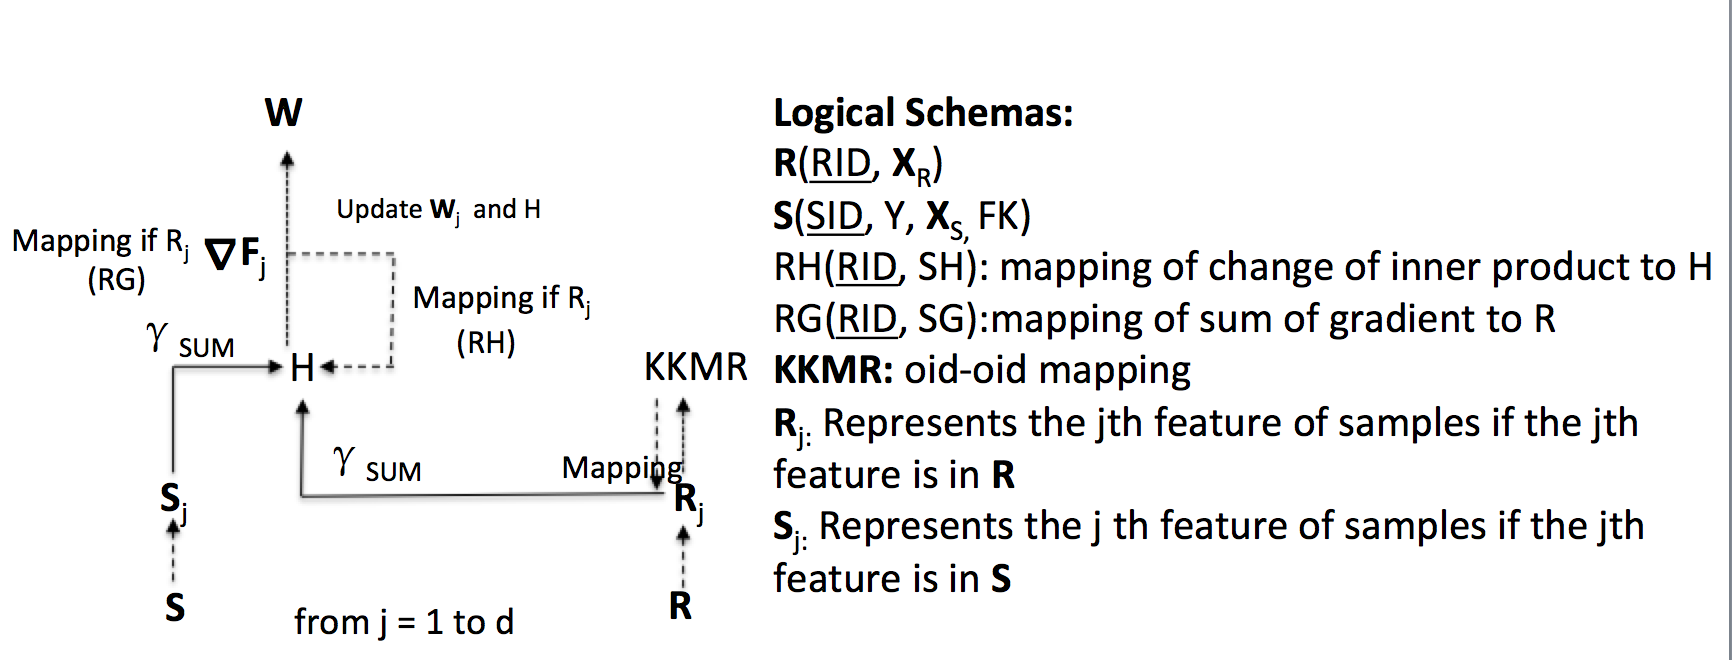
\includegraphics[height = 4cm, width = 8cm]{figs/FL.png}
\caption{Complete logical workflow of factorized learning. Considering feature column $S_j$ in \textbf{S}, simply calculate the partial gradient on corresponding column, and update the corresponding coordinate ($W_j$), and then update H. Considering feature column $R_j$ in \textbf{R}, look up the KKMR (oid-oid mapping) both in computation of the partial gradient (mapping called ``RG") and update of the residual vector H (mapping called ``RH"). Here, $\gamma_{SUM}$ denotes a \texttt{SUM} aggregation.
}
\label{fig:fl}
\end{figure}

The complete logical workflow and the corresponding logical schema of FL are shown in Figure~\ref{fig:fl}. 

%Step-by-Step explanation for FL 
\begin{enumerate}
\item
Before the iteration starts, compute KKMR (oid-oid mapping) with hash join and keep it in memory. Read column Y from \textbf{S} and keep it in memory
\item
When considering each feature column $S_j$ in \textbf{S}, there is no extra work: the procedure just works as what is described in \textbf{Algorithm 1}. Compute the partial gradient $\nabla F_j$ by summing up the partial coordinate gradient on $j_{th}$ feature of every sample. Update the corresponding coordinate $\textbf{W}_j$, and then update the residual vector H, which stores the inner product of each $\textbf{X}_{i,}$ and current model \textbf{W}. 
\item
When considering each feature column $R_j$ in \textbf{R}, to avoid the redundant computation, first map each partial gradient to every entry in \textbf{R} by looking up KKMR 
to get RG. After the mapping is done, compute the sum of corresponding partial gradient to every entry in RG  to get the \textit{full partial} gradient on $R_j$. Use the same way 
to get RH to avoid redundant computation of $\Delta W_j X_{(i,j})$ on same $X_{(i,j)}$. And then update the H by looking at the KKMR again to find the corresponding entry in 
RH.
\end{enumerate}

\begin{figure}[t]
\centering
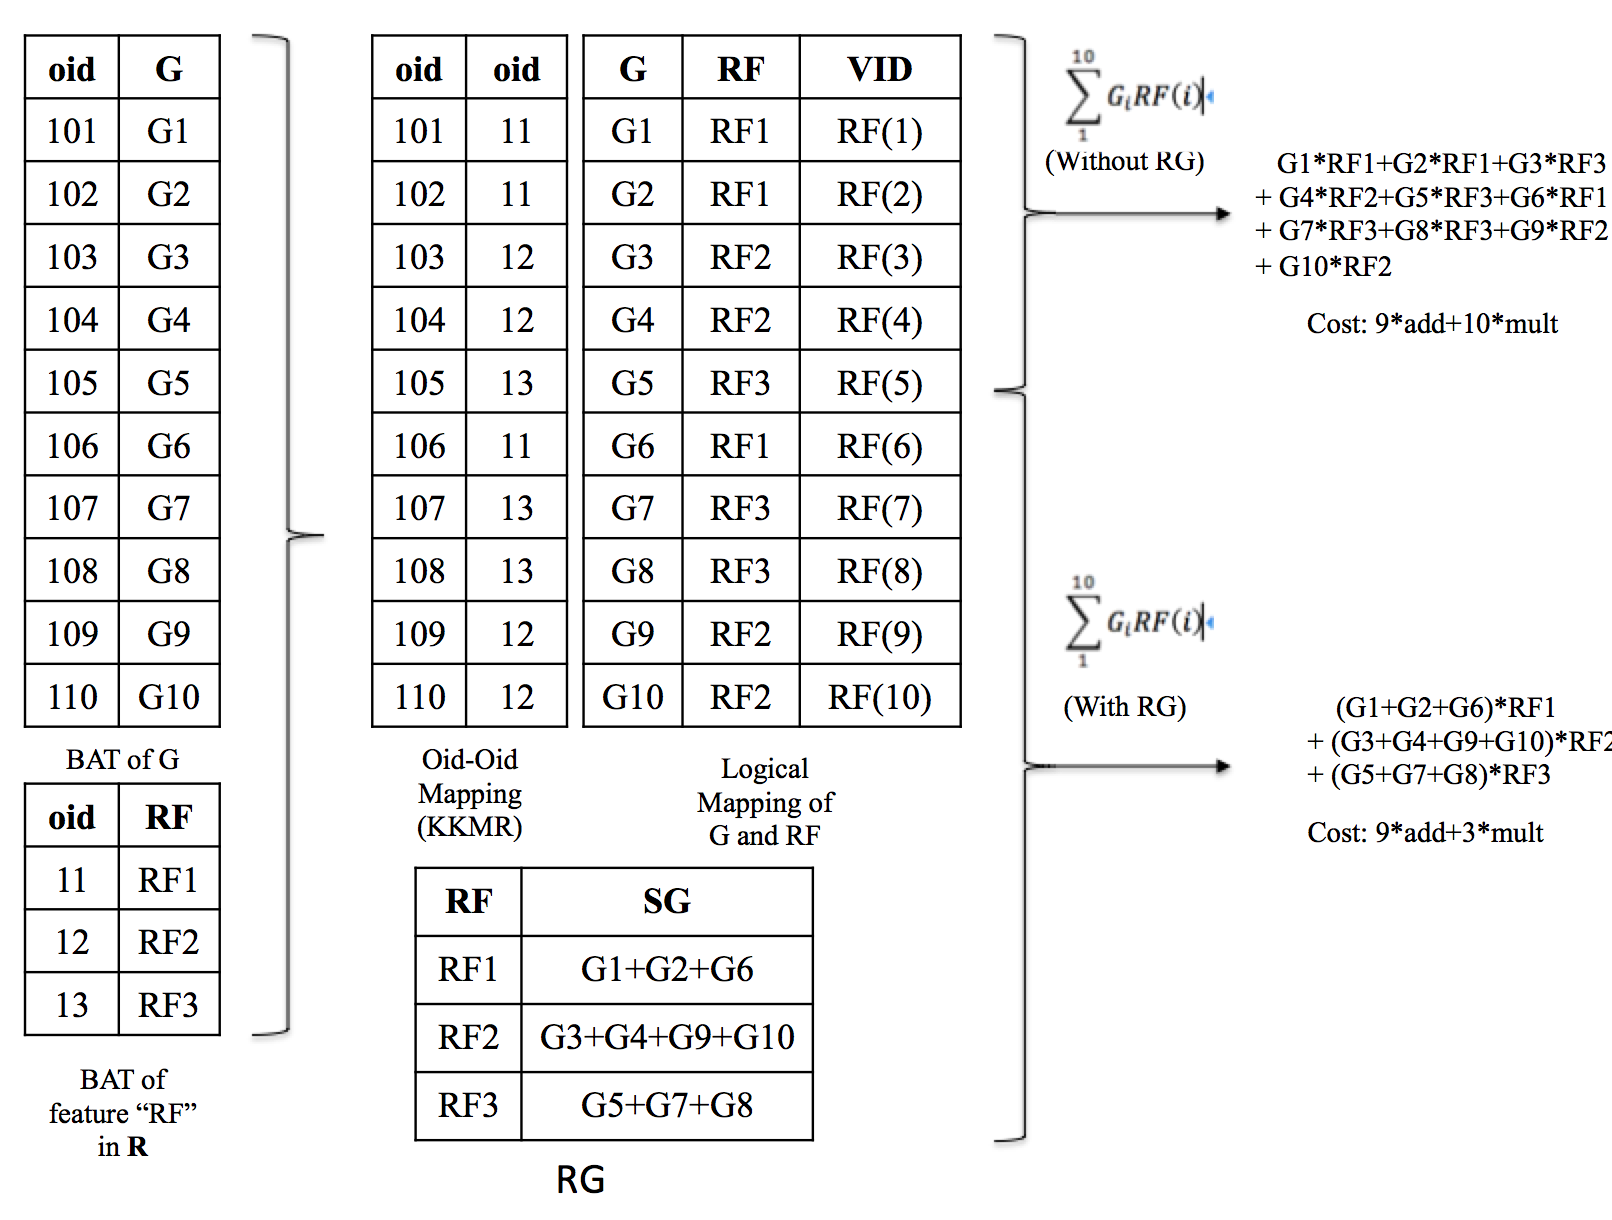
\includegraphics[height = 6cm]{figs/RG.png}
\caption{Considering a dataset with only ten samples (then the size of corresponding \textbf{S} is also ten), then the size of G is ten. Assume that the size of \textbf{R} is three, and one feature  in \textbf{R} is \textbf{RF}, then ``SG" for each entry RFj in \textbf{RF} is the sum of corresponding entries in G that map to RFj. 
}
\label{fig:RG}
\end{figure}

\begin{figure}[t]
\centering
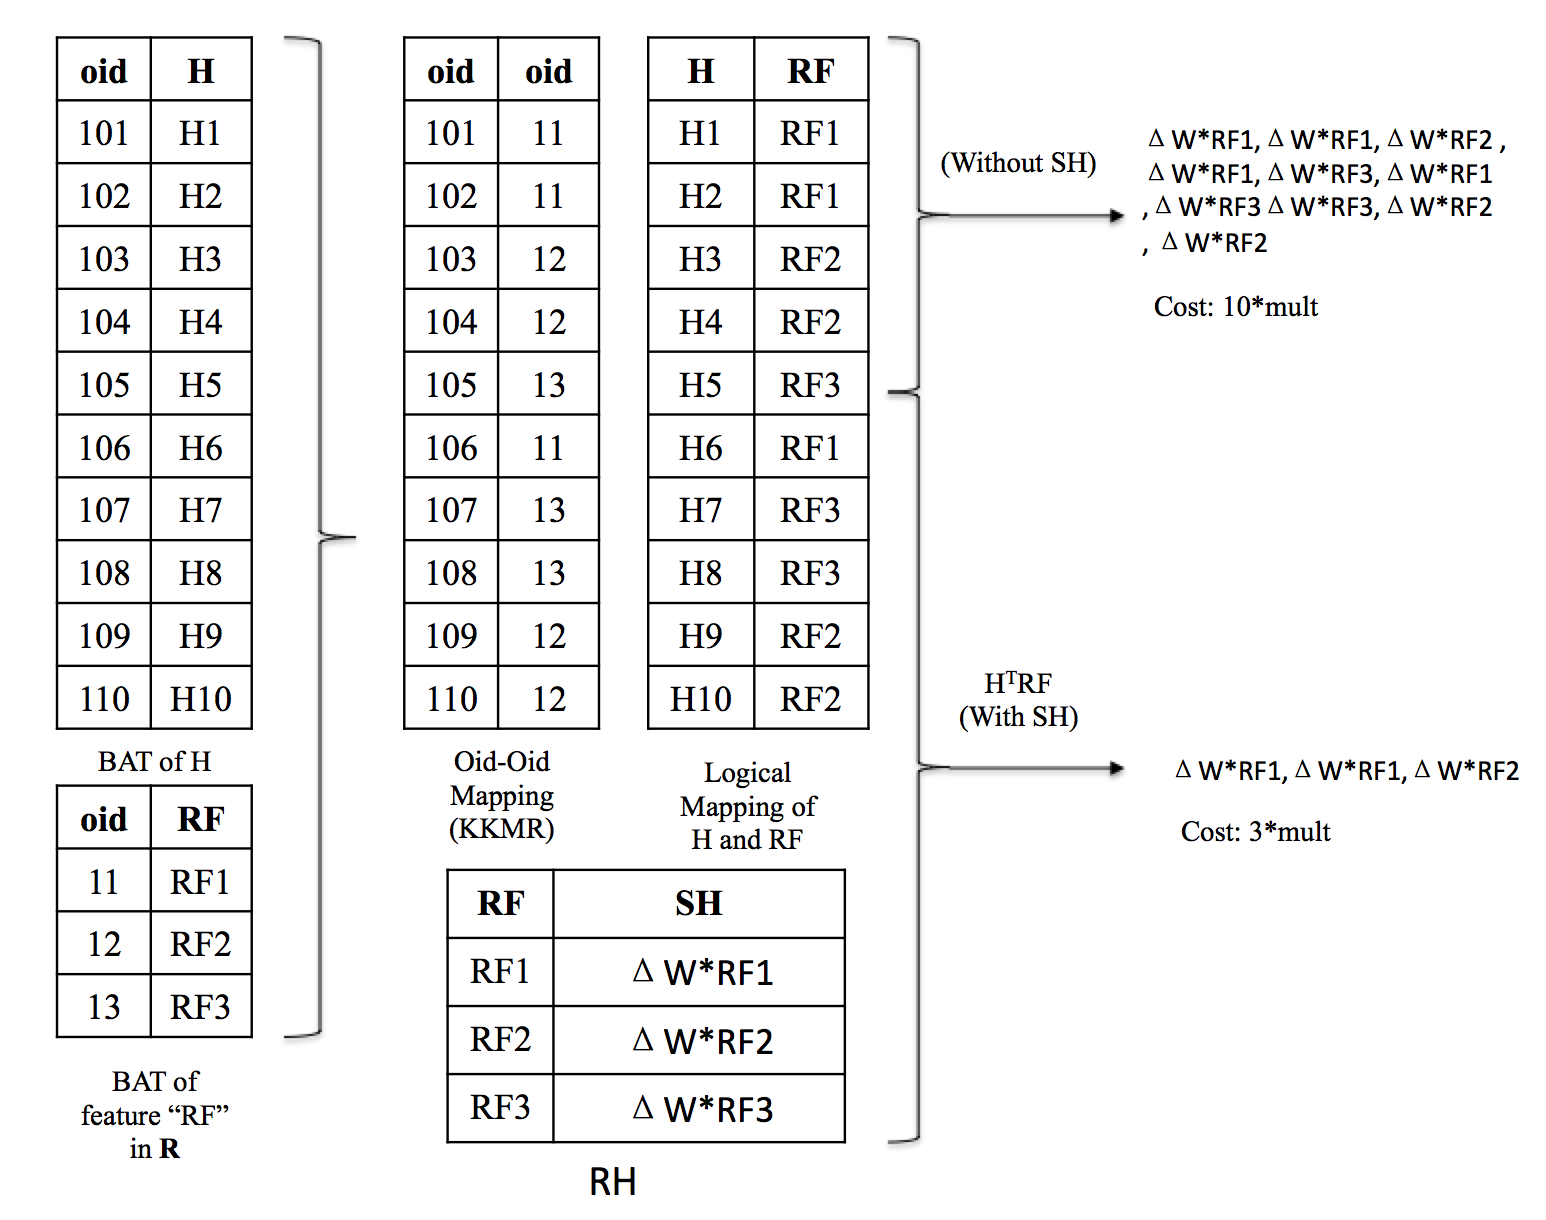
\includegraphics[height = 6cm]{figs/RH.png}
\caption{Considering a dataset with only ten samples (then the size of corresponding \textbf{S} is also ten ), then the size of H is ten. Assume that the size of \textbf{R} is three, and one feature  in \textbf{R} is \textbf{RF},
then ``SH" for each entry RFj in \textbf{RF} is the change of partial inner product on $X_{(,j)}$ that maps to RFj. 
}
\label{fig:RH}
\end{figure}

\vspace{-2mm}
\paragraph*{I/O Cost}
\vspace{-2mm}
\begin{alltt}
2|Scol| + |Rcol|      
+ Iters.[
	(dS-1).|Scol| + (dR-1).|Rcol| 
    ]
- (Iters-1).[                  
 min\{(dS-1).|Scol|+dR.|Rcol|, m - 4S|col|\}]   
\end{alltt}

\vspace{-2mm}
\paragraph*{CPU Cost}
\vspace{-3mm}
\begin{alltt}
  (nR+nS).hash             
+(nR+nS).copy
+ f.nS.comp
+ Iters.[
   	dR.[                    
	    nS.funcG           
	 + nR.mult      
	 + nS.add    
	 + 2*add+mult              
	 + nR.mult                 
	 + nS.add                  
	]
    + (dS-1)[           
            nS.funcG      
         + nS.(add+mult)
         + 2*add+mult      
         + nS.(add+mult)   
        ]  
        nS.(funcF+add)     	
   ]

\end{alltt}



\section{Conclusions}
This paragraph will end the body of this sample document.
Remember that you might still have Acknowledgments or
Appendices; brief samples of these
follow.  There is still the Bibliography to deal with; and
we will make a disclaimer about that here: with the exception
of the reference to the \LaTeX\ book, the citations in
this paper are to articles which have nothing to
do with the present subject and are used as
examples only.
%\end{document}  % This is where a 'short' article might terminate

% ensure same length columns on last page (might need two sub-sequent latex runs)
\balance

%ACKNOWLEDGMENTS are optional
\section{Acknowledgments}
This section is optional; it is a location for you
to acknowledge grants, funding, editing assistance and
what have you.  In the present case, for example, the
authors would like to thank Gerald Murray of ACM for
his help in codifying this \textit{Author's Guide}
and the \textbf{.cls} and \textbf{.tex} files that it describes.


% The following two commands are all you need in the
% initial runs of your .tex file to
% produce the bibliography for the citations in your paper.
\bibliographystyle{abbrv}
\bibliography{vldb_sample}  % vldb_sample.bib is the name of the Bibliography in this case
% You must have a proper ".bib" file
%  and remember to run:
% latex bibtex latex latex
% to resolve all references

\subsection{References}
Generated by bibtex from your ~.bib file.  Run latex,
then bibtex, then latex twice (to resolve references).

%APPENDIX is optional.
% ****************** APPENDIX **************************************
% Example of an appendix; typically would start on a new page
%pagebreak

\begin{appendix}
You can use an appendix for optional proofs or details of your evaluation which are not absolutely necessary to the core understanding of your paper. 

\section{Final Thoughts on Good Layout}
Please use readable font sizes in the figures and graphs. Avoid tempering with the correct border values, and the spacing (and format) of both text and captions of the PVLDB format (e.g. captions are bold).

At the end, please check for an overall pleasant layout, e.g. by ensuring a readable and logical positioning of any floating figures and tables. Please also check for any line overflows, which are only allowed in extraordinary circumstances (such as wide formulas or URLs where a line wrap would be counterintuitive).

Use the \texttt{balance} package together with a \texttt{\char'134 balance} command at the end of your document to ensure that the last page has balanced (i.e. same length) columns.

\end{appendix}



\end{document}
